\documentclass[10pt,twocolumn,letterpaper]{article}

\usepackage{cvpr}
\usepackage{times}
\usepackage{epsfig}
\usepackage{graphicx}
\usepackage{amsmath}
\usepackage{amssymb}
\usepackage{url}
\RequirePackage{framed}

% Include other packages here, before hyperref.

% If you comment hyperref and then uncomment it, you should delete
% egpaper.aux before re-running latex.  (Or just hit 'q' on the first latex
% run, let it finish, and you should be clear).
%\usepackage[pagebackref=true,breaklinks=true,letterpaper=true,colorlinks,bookmarks=false]{hyperref}

\cvprfinalcopy % *** Uncomment this line for the final submission

\def\cvprPaperID{****} % *** Enter the 3DV Paper ID here
\def\httilde{\mbox{\tt\raisebox{-.5ex}{\symbol{126}}}}

% Pages are numbered in submission mode, and unnumbered in camera-ready
\setcounter{page}{1}
\begin{document}

%%%%%%%%% TITLE
\title{3D Object Recognition with Deep Networks}

\author{Adrian Schneuwly\\
{\tt\small adrischn@ethz.ch}
\and
Johannes Oswald\\
{\tt\small voswaldj@eth.ch}
\and
Tobias Grundmann\\
{\tt\small tobiagru@ethz.ch}
}

\maketitle
% \thispagestyle{empty}

%%%%%%%%% ABSTRACT
\begin{abstract}
 
 %The increasing amount of LiDAR and RGBD cameras in e.g. mobile devices
 %  and robotic systems provide us with new information which can aid in various task including object
 %  recognition. In this paper we will discribe 3D Convolutional Deep Neural Networks and  how they are
 %  trained to recognize voxelized point cloud data from common objects.
   
  We implement 3D object recognition using a Convolutional Neural Network (CNN) approach. We adopt the network structure 
  outlined in \cite{voxnet} and implement it in Python using the Keras framework. We compare our trained CNN
  with the original paper and achieve similar positive results.

\end{abstract}
%%%%%%%%% BODY TEXT

\section{Introduction}

%One of the crucial tasks of computer systems based on visual information e.g. self-driving cars, autonomous robots, virtual
%enviroments ( Figure \ref{fig:obj_rec}) is to get a semantic understanding of the enviroment. Depth data has already proved its
%usability in obstacle avoidance or mapping but we want to investigate its potential to improve object recognition.

%Since Deep Learning dramatically improved state of the art object recognition \cite{cnn}, we will use Neural Networks to
%recognize objects from given point clouds. Especially the idea behind convolution in 2D Object recognition will be translated to our 
%3D data, resulting in a fast and accurate detector. 

Autonomous robotic systems like self-driving cars or drones operating in real world environments strongly depend on robust object recognition
in order to get a semantic understanding of the immediate surroundings.
Meanwhile, inexpensive depth data has become available with active range sensor such as LiDAR and RGBG cameras (e.g Google Tango). 
This information can aid in a wide range of tasks. While it is commonly used for obstacle avoidance and mapping, it is not fully 
utilized in the task of object recognition.


Machine learning approaches (Fig. \ref{fig:obj_rec}) in the form of Convolutional Neural Networks (CNN) dramatically improved state 
of the art image recognition \cite{krizhevsky2012imagenet}. Such networks learn the feature and classifiers from given training data.
While it is simple to extend this basic approach to volumetric data, it is not obvious what network structures will yield good performance.
VoxNet \cite{voxnet} is a fast basic 3D CNN architecture that makes use of the available depth information and achieves high object detection accuracy for 
3D point clouds.


\begin{figure}[h]
	\label{fig:obj_rec}
	\centering
	\frame{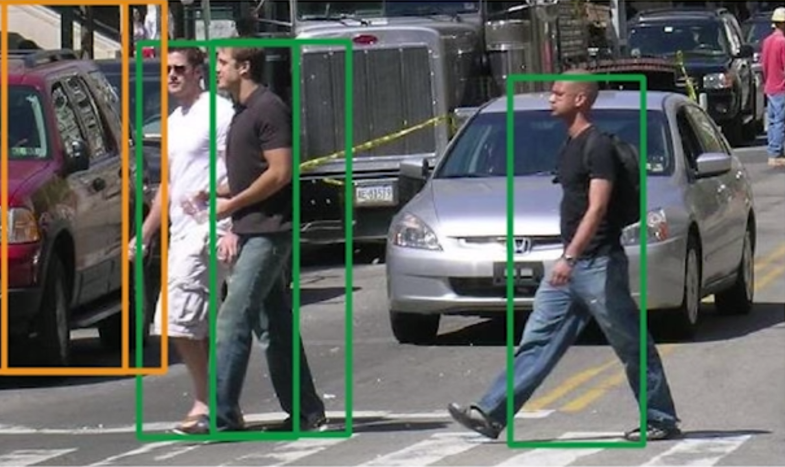
\includegraphics[width=0.45\textwidth]{figures/obj_rec}}
	\caption{Example of object recognitions: Detection as binary classification problem (pedestrian vs no pedestrian). Slide over all possible locations in the image and classify patches. 
	  (Image source: \cite{udacity})}
\end{figure}

%-------------------------------------------------------------------------

\section{Related Work}

This section is strongly based on the 'Related Work' section of VoxNet paper \cite{voxnet}.
%On the one hand, there is a large body of work of object recognition using 3D point clouds but not making use of Neural Networks. 
%Mostly methods combine hand-crafted features or descriptors with a machine learning classifier ([10], [11], [12]). 
%Similiar methods are seen with semantic segmentation, with structured output classifiers instead of single output classifiers ([14], [15], [16]).

%On the other hand 2.5D CNNs were used for object recognition but fail to make full use of geometric information in the data. T
%heir approaches simply treat the depth channel as an additional channel, along with the RGB channels. ([17], [18], [19], [20]) 

%Additionally, 3D CNNs already proved there usability in video analysis ([23], [24]). In this case, time acts as the third dimension but algorithmically, 
%these architectures work the same as ours, but the nature of the data is very different.


\subsection{Object Recognition with Point Cloud Data}
Various publications on both semantic segmentation \cite{koppula2011semantic} and object recognition 
(\cite{teichman2011towards}, \cite{golovinskiy2009shape}) using 3D point clouds from LiDAR or RGBD sensors are available. 
Most of this work uses a pipeline combining hand-crafted features or descriptors with a machine learning classifier.
The VoxNet architecture on the other hand learns to extract features and classify objects from the raw volumetric data.


\subsection{3D  Convolutional Neural Networks}
RBG image object recognition has been dramatically improved by Convolutional Neural Networks.
Building on that success, several authors have extended that basic approach to RBGD, simply treating the depth as 
an additional channel (\cite{hoft2014fast}, \cite{socher2012convolutional}). While straightforward, this approach does not
make full use of the geometric information available in the data.
In contrast, the fully volumetric representation described in \cite{voxnet} takes advantage of that information.
This volumetric representation is richer as it also distinguishes free space from unknown space.

Additionally, CNN architectures with volumetric (3D) convolutions have already proven their usability in video analysis \cite{ji20133d}. In this
case time acts as the third dimension. 
In the RBGD domain, \cite{shape} proposes ``a convolutional deep belief network to represent geometric 3D shape as a probability distribution of binary variables on a 3D voxel grid.''
Their model can jointly recognize and reconstruct objects from a single view. In order to train the deep belief network the authors constructed the 
3D CAD model dataset called ModelNet (see section \ref{data:modelnet}).


\section{Convolutional Neural Networks}

At the core of a neural network is a logistic classifier. 
%For given data, we train weights and bias of a linear equation which will then be transformed into 
%probabilities by using a softmax function. Figure \ref{fig:classifier}.
Weights and bias of a linear equation are trained on provided data. Inserting an input to the system yields an output, which is
transformed into probabilities by using a softmax function. See Figure \ref{fig:classifier}.

\begin{figure}[h]
	\label{fig:classifier}
	\centering
	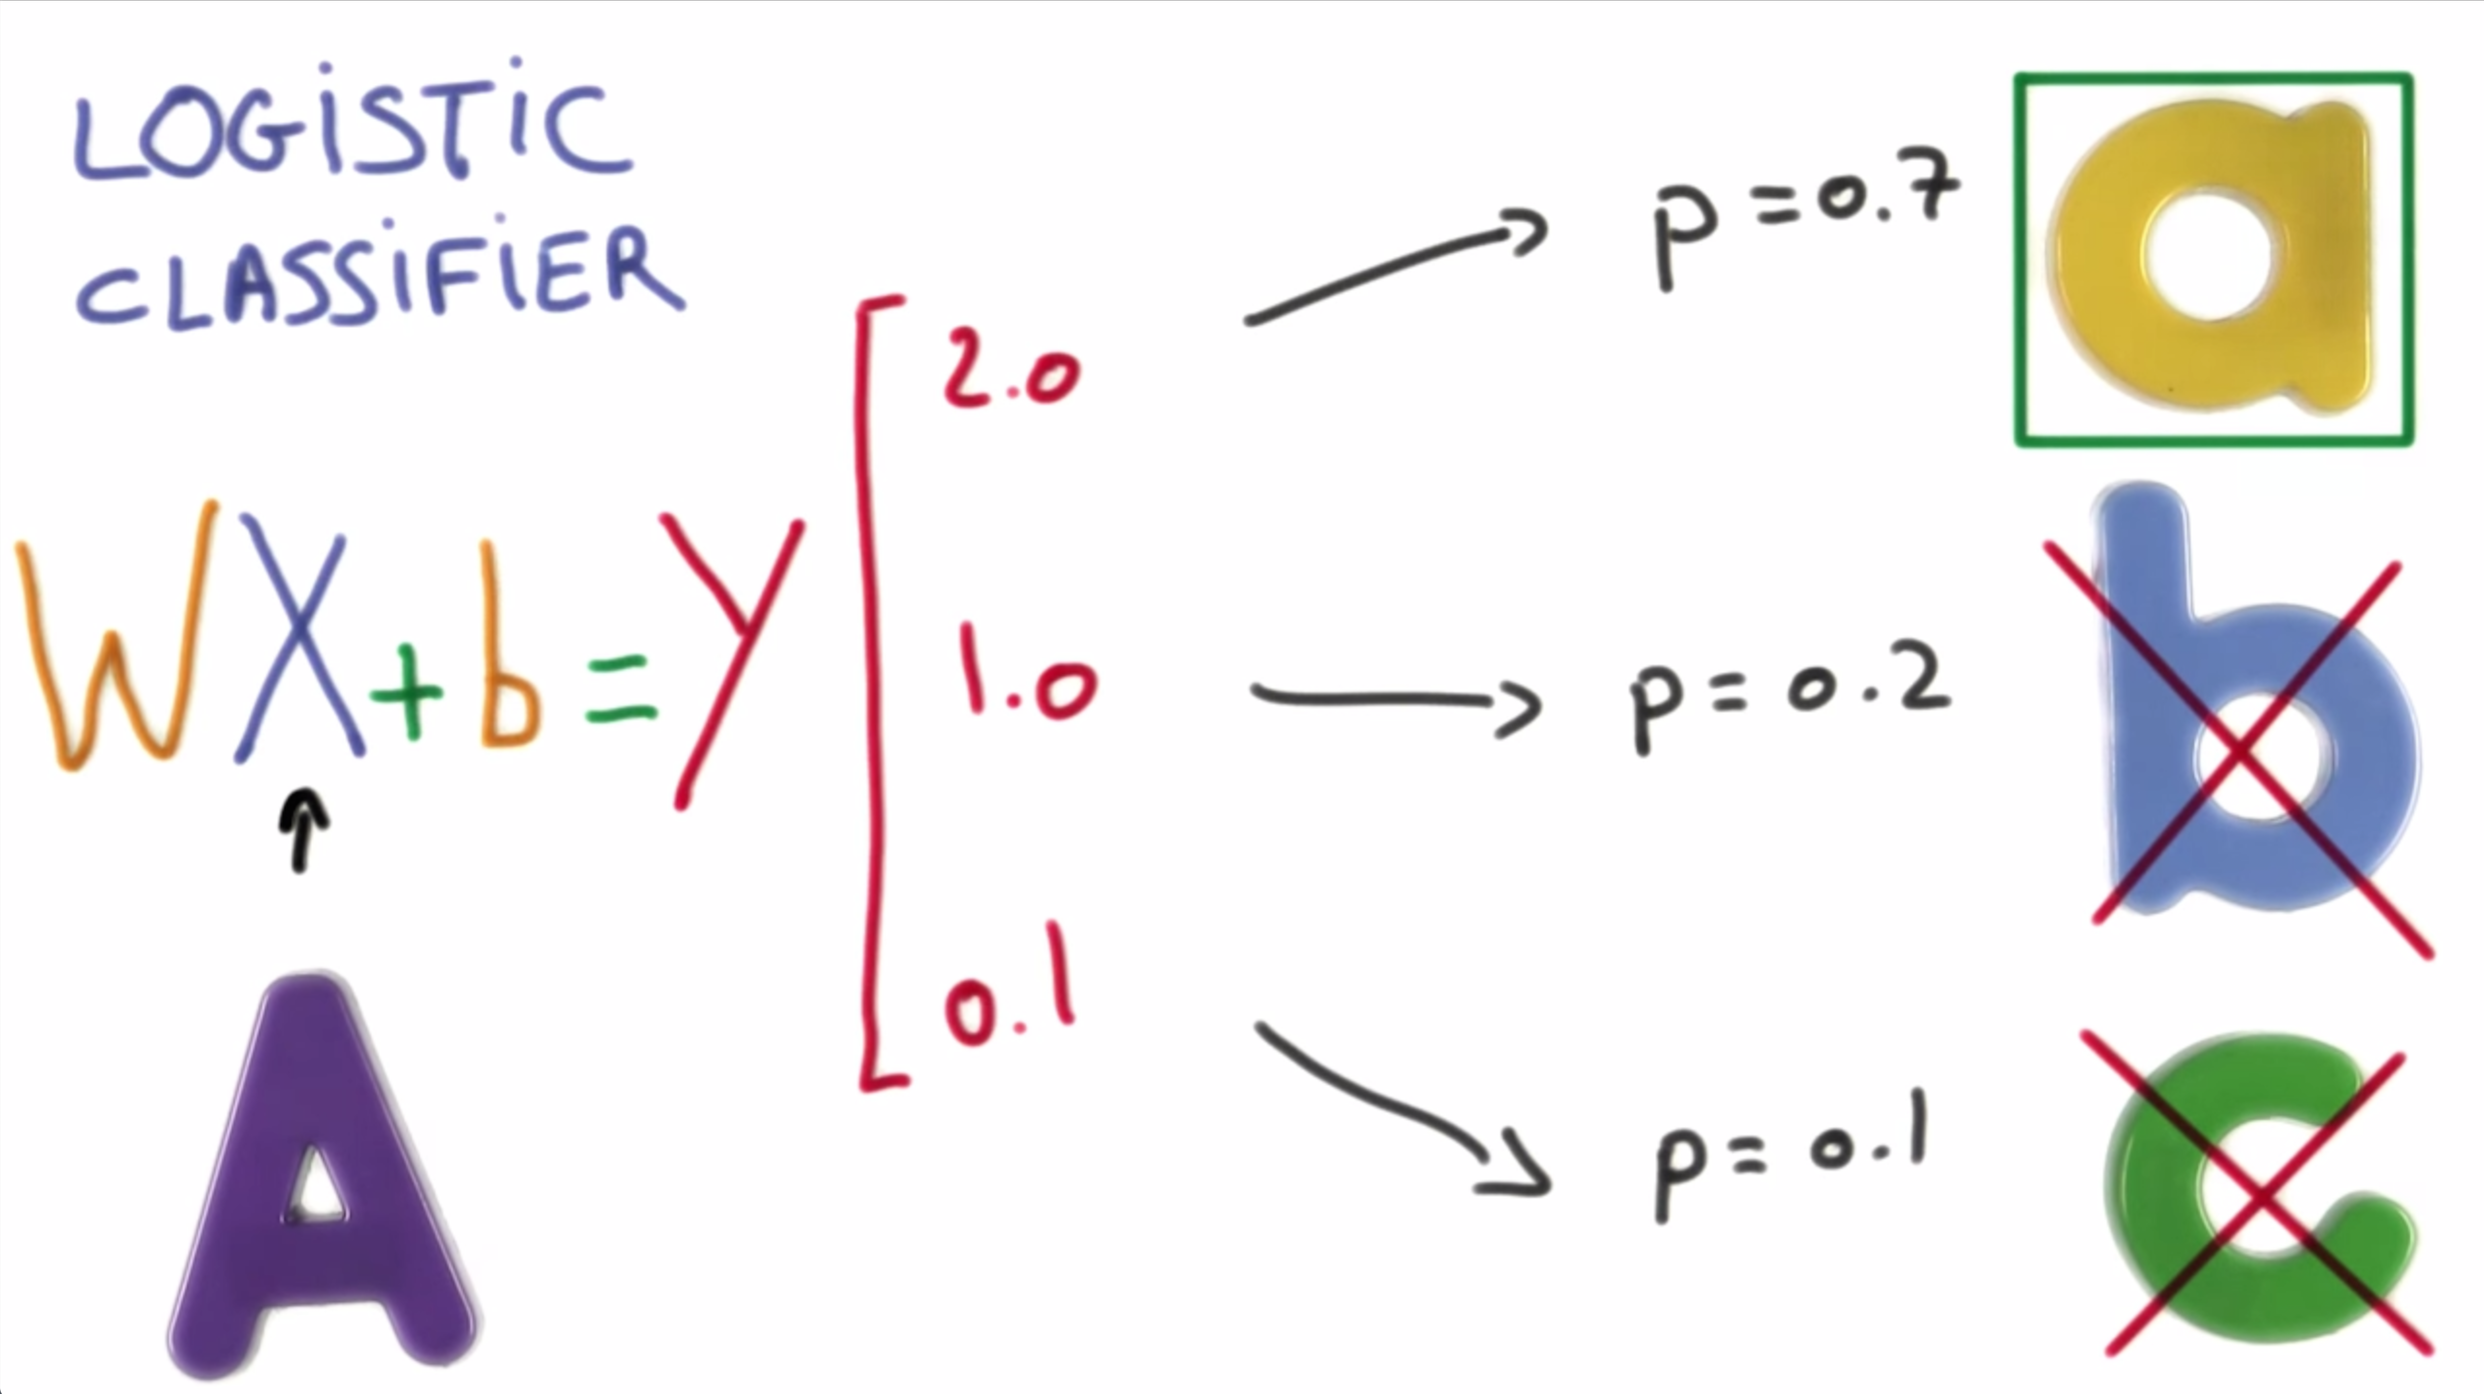
\includegraphics[width=0.45\textwidth]{figures/classifier}
	\caption{Weights W and bias b are trained to classify an input. If the letter 'A' is feed to the network,
	it is classified as an 'A' with a certainty of 0.7. (image source: \cite{udacity})}
\end{figure}

Linear Neural Networks are limited and therefore CNNs are advanced by non-linear feature maps which \textit{deepen} 
when successively applied. The deep neural network of \cite{voxnet} uses convolutions and max-pooling.
For convolutions, we run small neural networks with given output size / depth on a patch which walks through the 3D data. 
When leaving out / jumping voxels (striding),
the spatial dimension is squeezed while extracting local features of the given object. 
Through repeating this procedure we arrive at an output depth which corresponds to the semantic complexity of the object recognition task. 

\begin{figure}[h]
	\label{fig:convolution}
	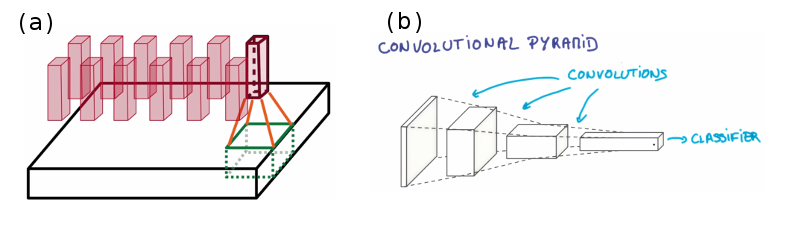
\includegraphics[width=0.45\textwidth]{figures/conv}
	\caption{(a) patch with stride 2 (b) multiple convolutions. (image source: \cite{udacity})}
\end{figure}

The second technique to deepen a network is pooling. Instead of striding to squeeze the dimension, 
we can extract for example the maximum of a patch and thereby reduce the spatial dimension. 
See Figure \ref{fig:voxnet_structure} for a detailed description of the model used in our approach.

\begin{figure}[h]
	\label{fig:pooling}
	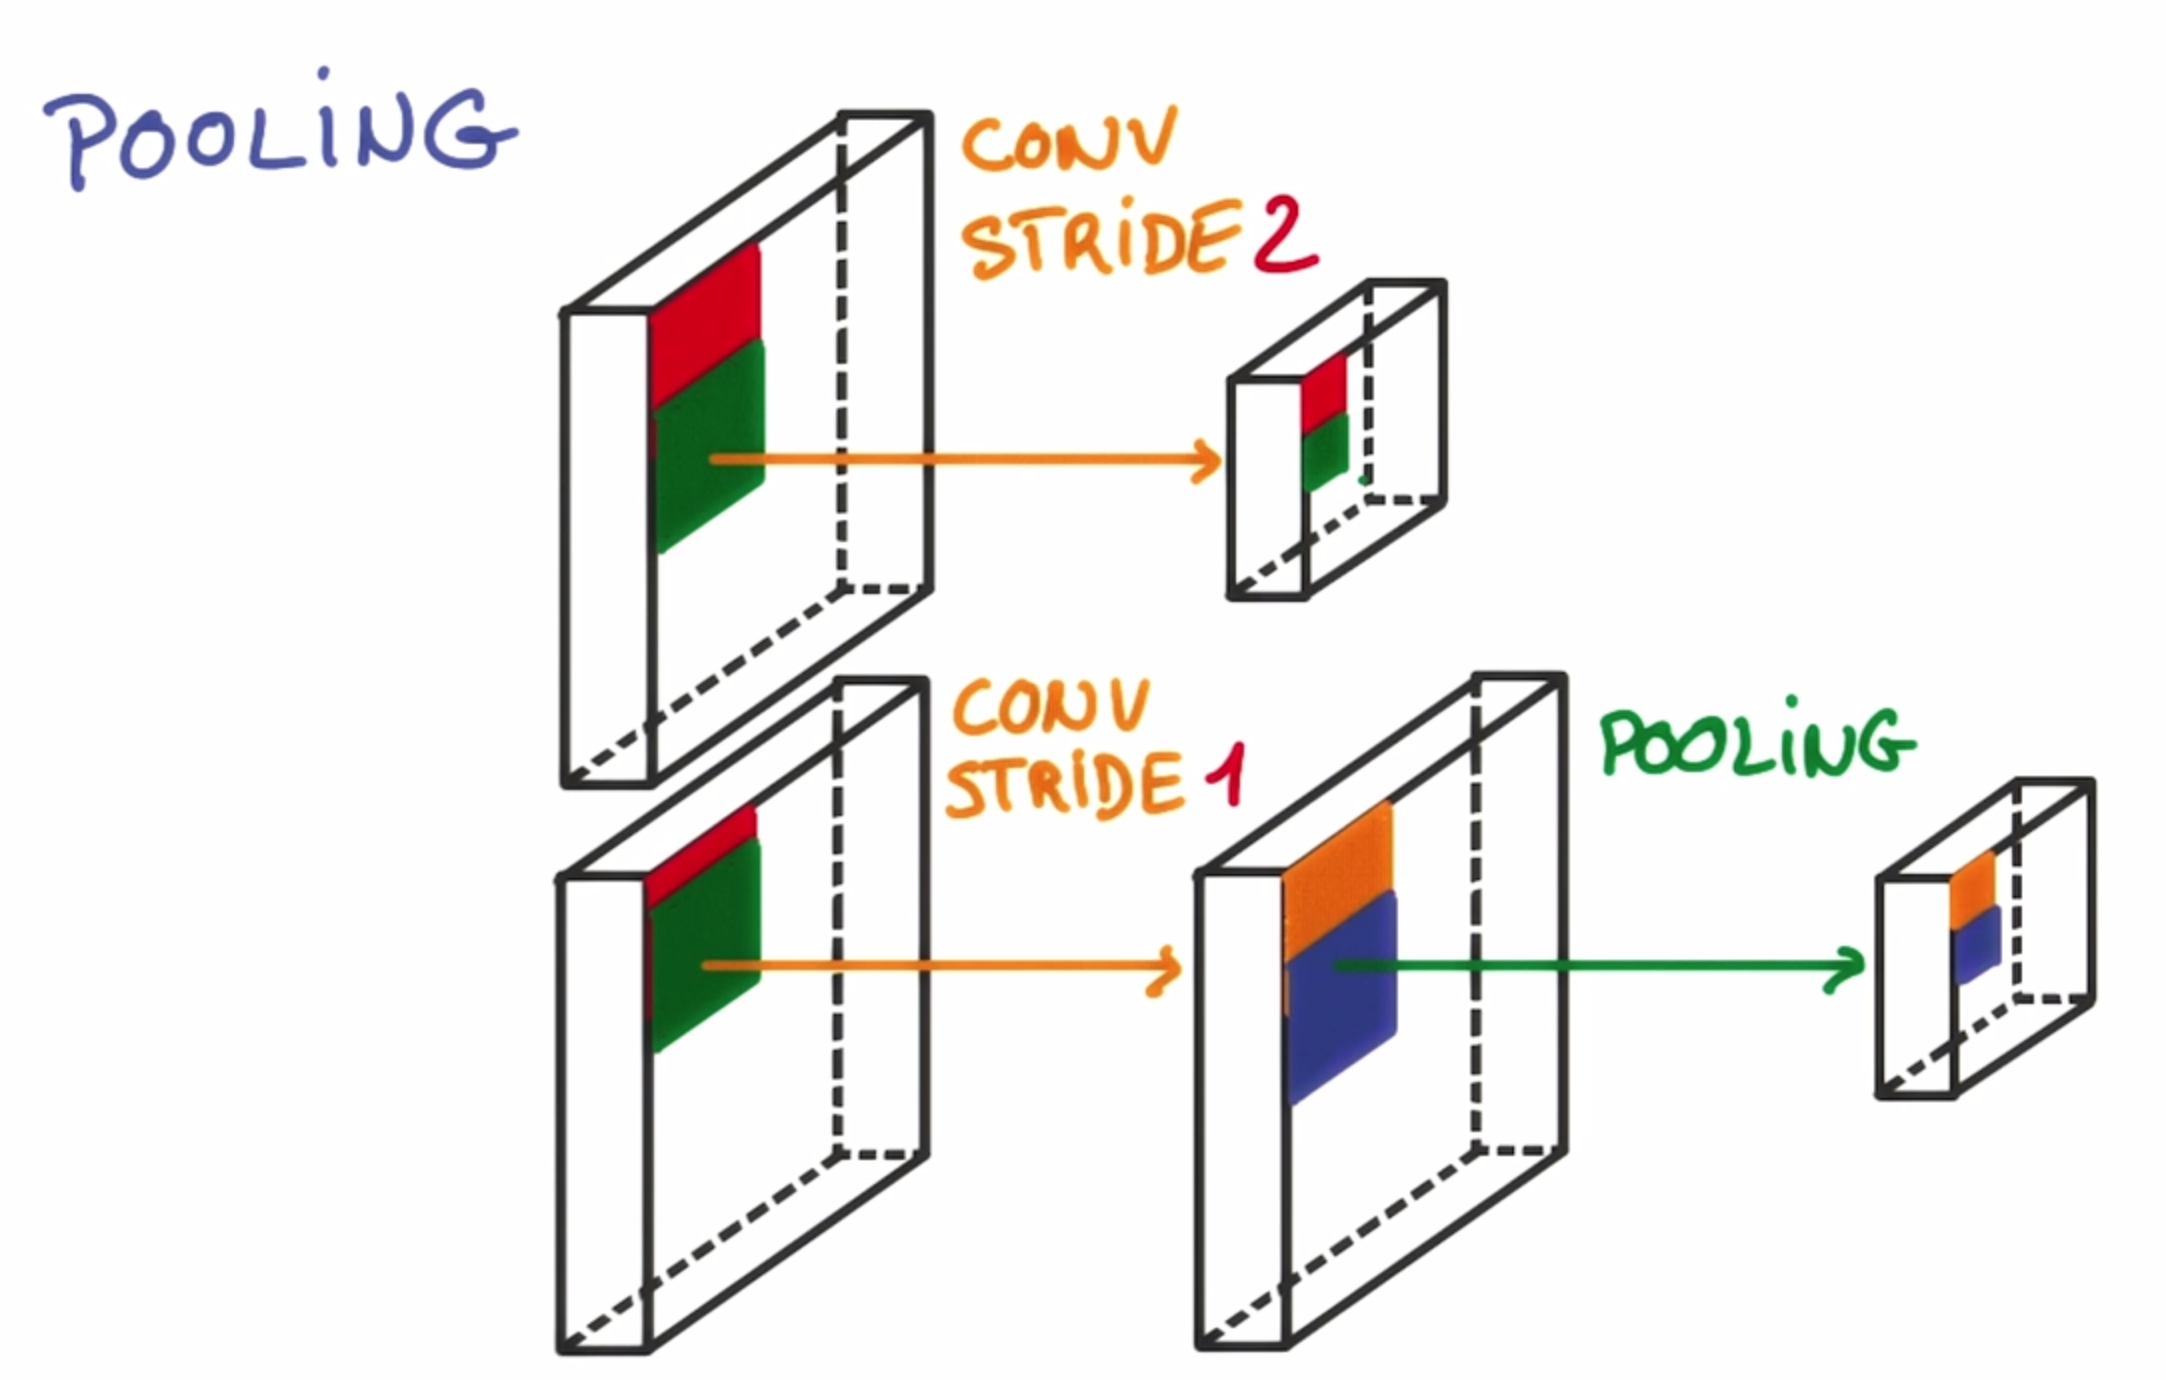
\includegraphics[width=0.25\textwidth]{figures/con_max}
	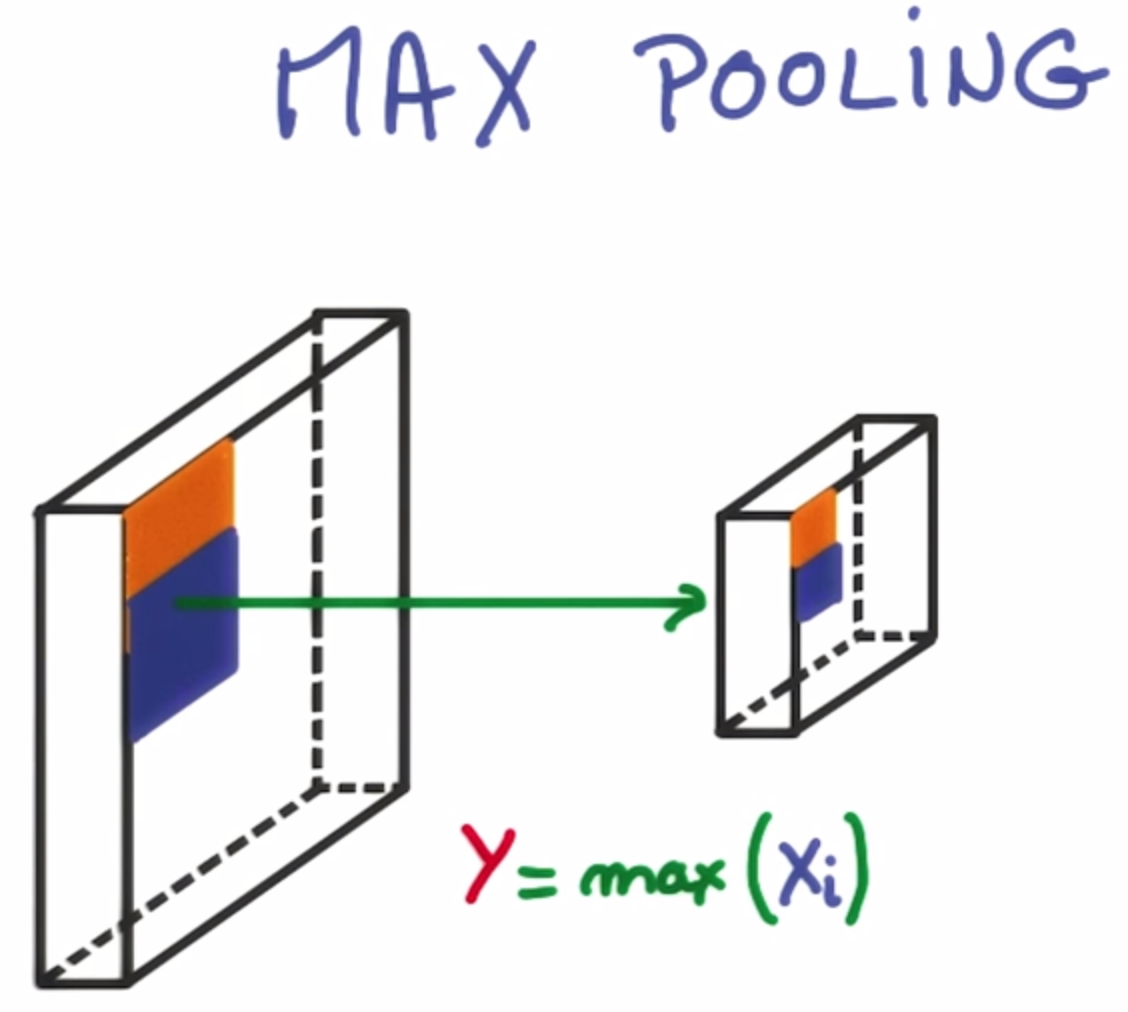
\includegraphics[width=0.16\textwidth]{figures/max}
	\caption{left: stride 2 vs. stride 1 + Pooling \quad right: max-pooling (image source: \cite{udacity})}
\end{figure}

In order to train our model, we also have to test how well it is doing during and after training. 
Validating the model on training data does not work since the model remembers all its input. 
Therefore we split the original data into a test and training set which enables us to check how well the 
classifier performs on unknown data. It is common phenomenon that a complex model fits a given 
dataset, but fails to generalize on new data. This is called \textit{overfitting}.

\section{Datasets}
\label{data:modelnet}

In order for a CNN to perform well, the amount of training data needs to be sufficiently large. One large scale 3D CAD dataset is Princeton's 
ModelNet \cite{shape}. The dataset was constructed by querying common object categories from the SUN database \cite{sun} and 
by collecting 3D CAD models through online search engines. Human workers on Amazon Mechanical Turk were hired 
to manually validate the class labels assigned to each object.

The subset ModelNet40 is a collection of the 40 most common object categories with 100 unique CAD models each. The data is further augmented
by rotating each model by 30 degrees along the gravity direction (12 poses per model). 
The ModelNet40 data is available online in a voxelized version. The grid size is 30x30x30 with 1 extra cell of padding in both directions.

\section{Implementation: VoxNet \cite{voxnet}}

\textit{In the following, parts contributed by author Adrian/Johannes/Tobias will be labeled 
as A1/A2/A3.}\newline

The overall goal of the project is to classify an object from a given 3D point cloud. Figure \ref{fig:algo} outlines 
the required pipeline.

\begin{figure}[h]
	\label{fig:algo}
	\centering
	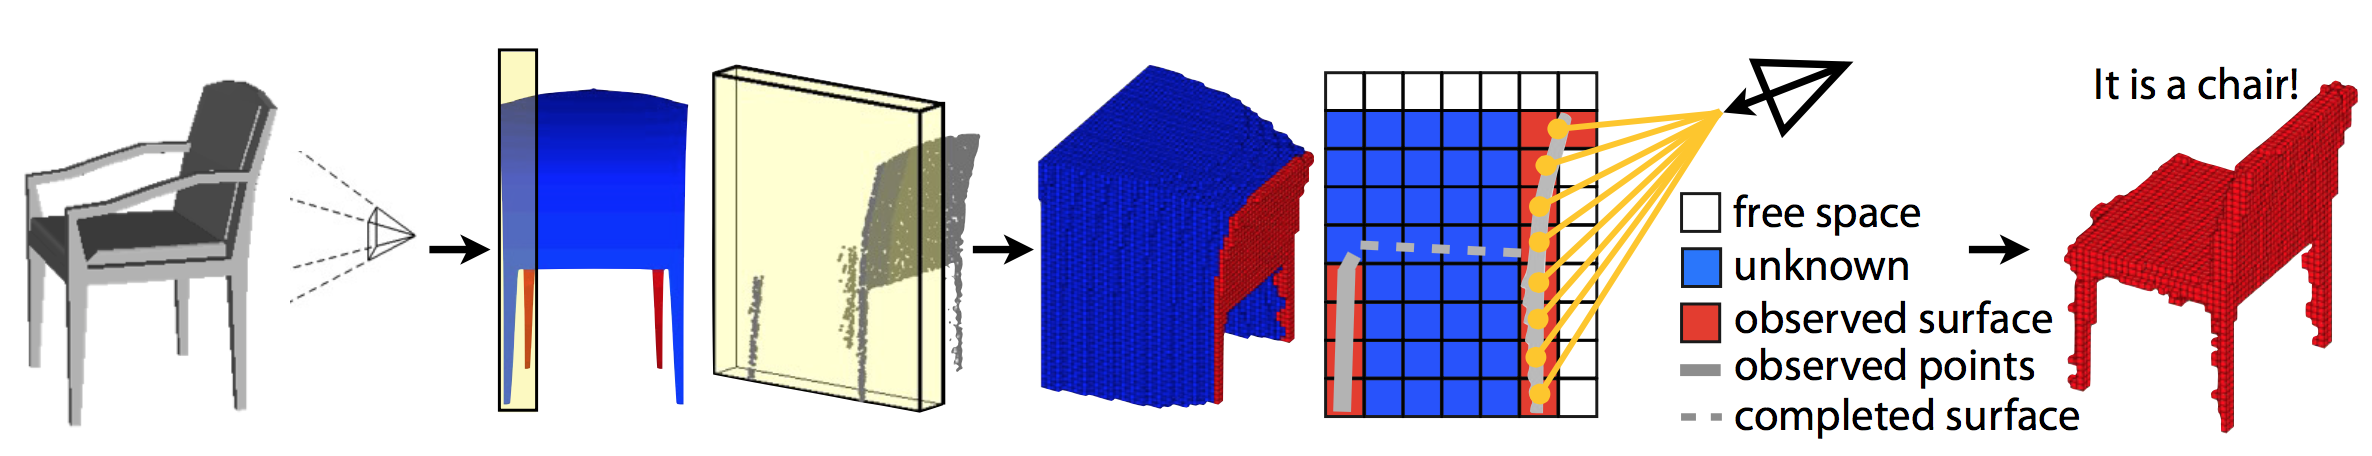
\includegraphics[width=0.5\textwidth]{figures/algo}
	\caption{ Depth and point cloud are converted to voxels and then feed to the network 
	for classification. (source: \cite{shape})}
\end{figure}

The voxelized version of ModelNet40 is provided in the form of Matlab (.mat) files, where every single CAD model is stored 
in a separate file.

In a first step, A3 converted the data to the hdf5 format and stored all the model data in a single file in order to overcome 
the cumbersome character of the provided file structure. The hdf5 format not only compresses the data size dramatically, but also enables
very simple data access. 
Next, A2/A3 implemented (in Python) a model data handling library, which can load the voxel grids from the hdf5. Generally, during the loading 
process the model set is split into two parts, a training and validation set. The responsibility of the library is to prepare 
the voxel arrays for the CNN, including shuffling and splitting the data into batches.

The second part is the Convolutional Neural Network (Figure \ref{fig:voxnet_structure}) itself, which was implemented (in Python) by A1/A2.
In a first attempt the TensorFlow framework was used, until we realized that at this point in time the framework 
did not support 3D convolutions. As an alternative the highly modular deep learning library Keras on top of Theano
was chosen for the implementation.

\begin{figure}[h]
	\label{fig:voxnet_structure}
	\centering
	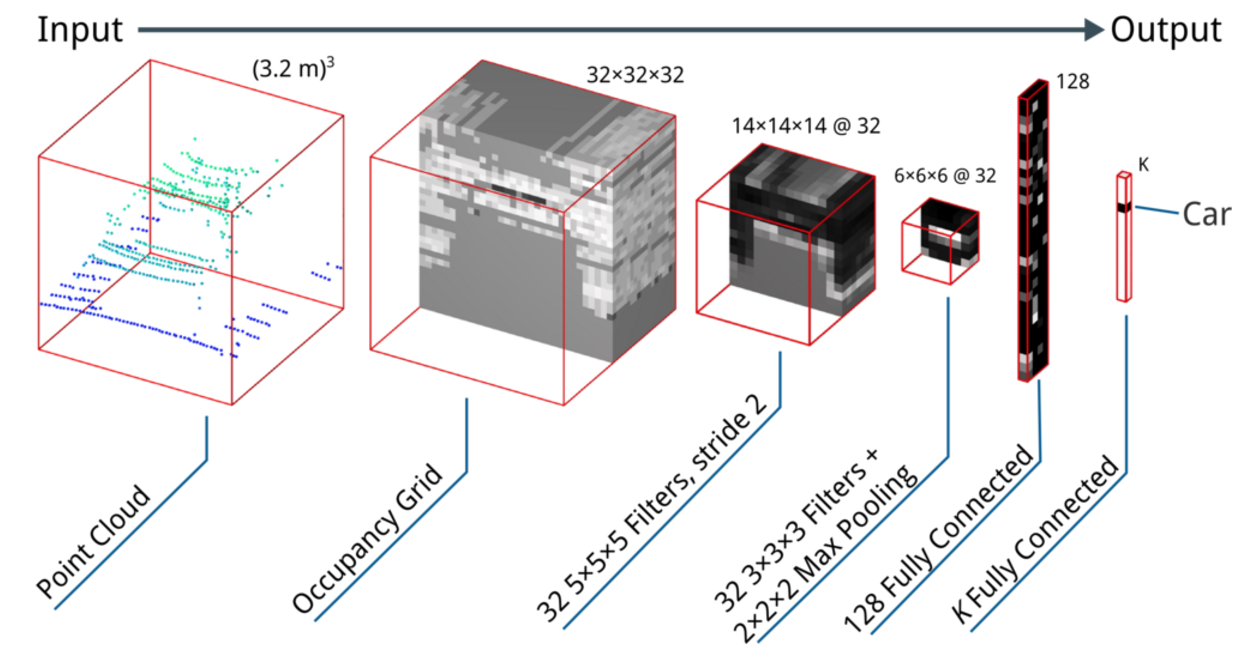
\includegraphics[width=0.45\textwidth]{figures/model}
	\caption{VoxNet layer architecture. Two successive convolutions followed by 
	max-pooling and fully connected layers (source: \cite{mature})}
\end{figure}

The training environment was set up and used by all the authors. 

 
\section{Training}

The training process takes around 9 to 20 hours on a NVIDIA GTX 980TI (6GB) GPU, using CUDA 7.5 and cuDNN 5, 
depending on the choice of the dataset (ModelNet10/40). Any methods to improve the score by further data augmentation,
such as the random augmentation and multi resolution where not implemented as the amount of GPU time available
was very limited. This might affect the results of the score. 
The implementation does not make use of early stopping as we are using dropout and weight regulizers,
thus avoiding overfitting by the use of early stopping, would not show any improvements.
This was tested and proven to be true. Any attempts of improving the score by tuning the learning rate have not show to be successful.
Common to best practice weights are saved after every epoch of training to avoid loss of data.

\section{Results}

Our implementation achieved very good results for the small data set but failed to achieve the excellent score of the 
original VoxNet implementation on the larger ModelNet40. One possible explanation could be the slightly different setup due 
to different libraries used in our implementation. 
A detail missed in the reimplemenation is the data augmentation done by \cite{voxnet}. 
They randomly added perturbed copies of instances during the training to enhance versatility of the data.
Additionally, more time to fine tune sizes of test/training set could have improved the performance and reduced overfitting.

\begin{center}
\begin{tabular}{ |p{2.3cm}||p{2.3cm}|p{2.3cm}|  }
 \hline
 Algorithm & ModelNet10 Classification Accuracy  & ModelNet40 Classification Accuracy \\
 \hline
 VoxNet \cite{voxnet}   & 83\% & 92\% \\
 3DShapeNets  \cite{shape}   & 77 \% & 83.5\% \\
\textbf{ETH VoxNet}    & \textbf{81.8\%}   & \textbf{82.3 \%}  \\
 \hline
\end{tabular}
\end{center}

\vspace{0.3cm}
The trained network was also tested on data acquired with Google Tango. The point clouds were first voxelized
and shaped into the right format to feed into the network. We feed voxels of 3 different objects/scenes: Chair, 
stool (Figure \ref{fig:voxel_stool}) and a desk scene (Figure \ref{fig:desk}). Both single objects (chair, 
stool) get recognized with very high accuracy of over 98\%.

%TODO image ränder abschneiden (weniger weiss)
\begin{figure}[h]
	\label{fig:voxel_stool}
	\centering
	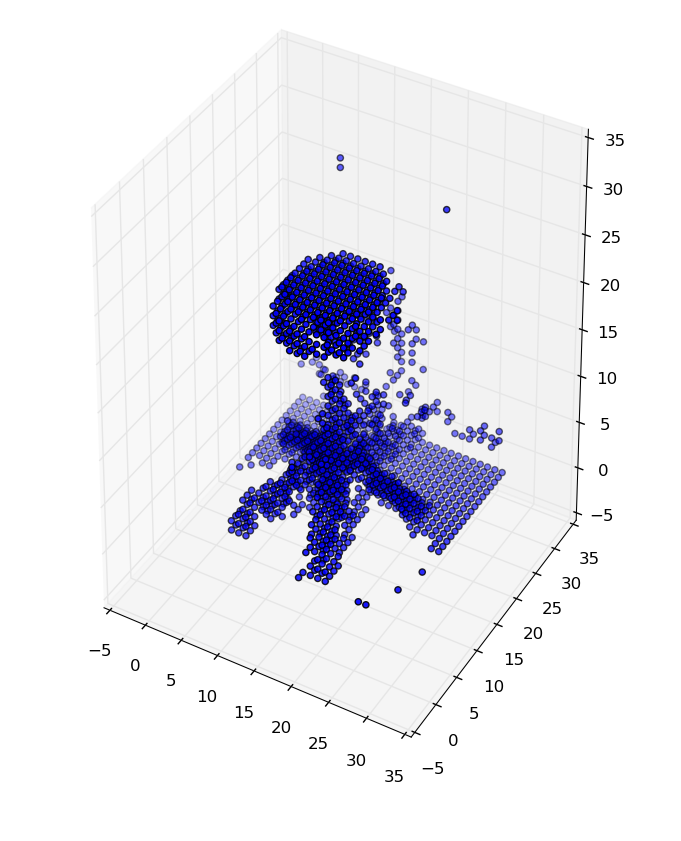
\includegraphics[width=0.42\textwidth]{figures/tango_voxel_stool}
	\caption{Voxelized stool}
\end{figure}

\begin{figure}[h]
	\label{fig:desk}
	\centering
	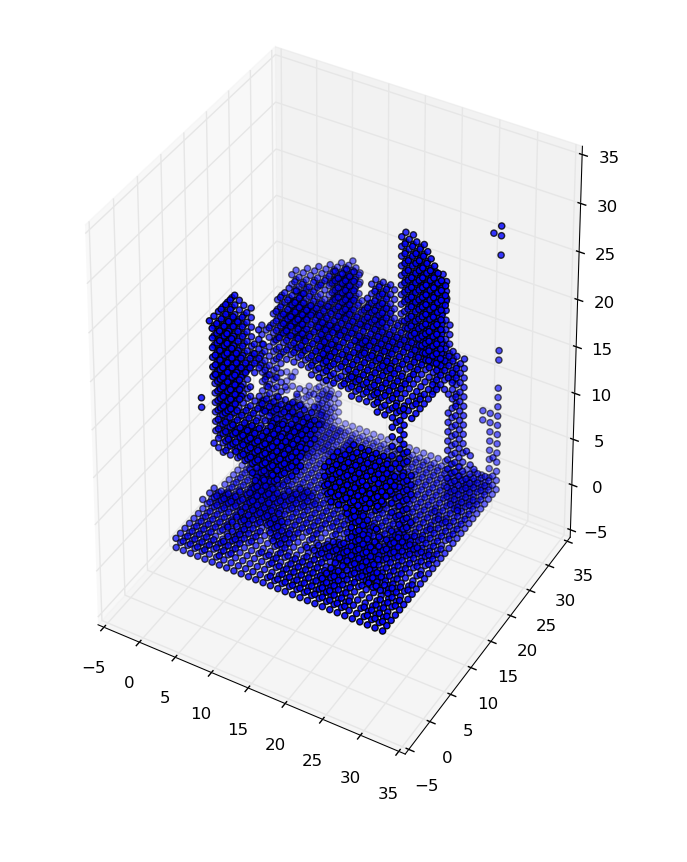
\includegraphics[width=0.42\textwidth]{figures/tango_voxel_desk_scene}
	\caption{Voxelized desk \textbf{source ????? martin ?}}
\end{figure}

The systems is designed to distinguish between single object and therefore not surprisingly fails when
tested on e.g. a desk scene includuing multiple objects e.g. chair, desk, display (Fig. \ref{fig:desk}).

\section{Conclusion}

The team successfully reimplemented a very clean and working VoxNet with comparable results.
After voxelizing point cloud data from e.g. LiDAR or RGBD, the system is capable of efficient and accurate object classification in real time. 

\section{Outline}
Due to fine tuning and implementation of the data augementation used by \cite{voxnet}, same results even on the larger ModelNet40 
should be achieve quickly. One failure of the system is the difficulty when working with multi object inputs., Fig. \ref{fig:desk}. 
When implementing the system on e.g. Google Tango, one would first need a object extraction from the scene and additionally rescaling into the used voxel grid size to use the implemented classifier. 

{\small
\bibliographystyle{ieee}
\bibliography{reference}
}

\end{document}
